\section{Zusammenfassung und Ausblick}

\begin{frame}
\frametitle{Zusammenfassung}
Wir haben kennengelernt:
\begin{itemize}
\item verschiedene Datentypen (tw. \glqq High Level\grqq)
\item die wichtigsten Statements
\item Funktionsdeklaration und -Benutzung
\item Module und Pakete
\item Fehler und Ausnahmen, Behandlung selbiger
\item objektorientierte Programmierung
\item einige h"aufig verwendete Standardmodule
\end{itemize}
\end{frame}

\begin{frame}
\frametitle{Offene Punkte}
Nicht behandelte, tw. fortgeschrittene Themen:
\begin{itemize}
\item funktionale Techniken mit Listen: List Comprehensions, \texttt{filter()}, \texttt{map()}, \texttt{reduce()}
\item Lambda-Funktionen, Funktionen mit variablen Parametern
\item Iteratoren, Generatoren
\item Closures, Dekoratoren (Funktionswrapper)
\item Ausnutzung von Pythons Dynamik:\\\texttt{getattr}, \texttt{setattr}, Metaklassen, \dots
\item Weitere Standardmodule: Mail, HTML, XML, Zeit\&Datum, Profiling, Debugging, Unittesting, \dots
\item Third Party-Module:\\GUI, Grafik, Webprogrammierung, Datenbanken, \dots
\end{itemize}
\end{frame}

\begin{frame}
\frametitle{Grafische Benutzeroberfl"achen}
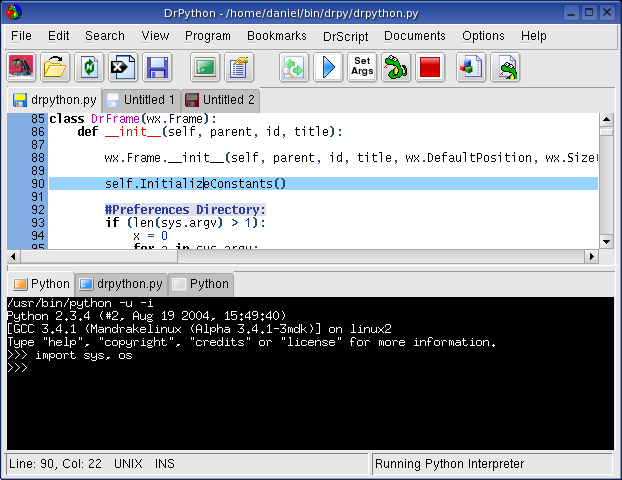
\includegraphics[height=4.3cm]{images/drpython_screenshot.png}
\hspace*{2mm}
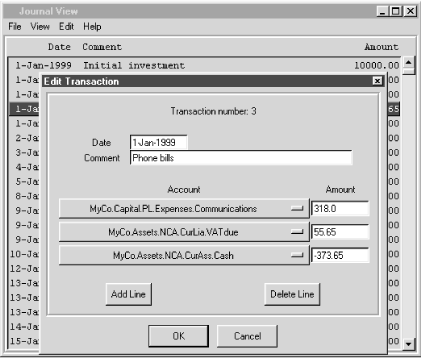
\includegraphics[height=4.3cm]{images/tkinter.png}

\begin{itemize}
\item Tk (aus Standardbibliothek)
\item wxWidgets (GUI-Toolkit je nach Betriebssystem)
\item GTK
\item QT
\end{itemize}
\end{frame}

\begin{frame}
\frametitle{Web-Programmierung}
\begin{itemize}
\item CGI-Scripte: Modul \texttt{cgi} aus  Standardbibliothek
\item Webframeworks: Django, TurboGears, Pylons, \dots
\item Templatesysteme: Cheetah, Genshi, Jinja, \dots
\item Content Management Systeme (CMS): Zope, Plone, Skeletonz, \dots
\item Wikis: MoinMoin, \dots
\end{itemize}

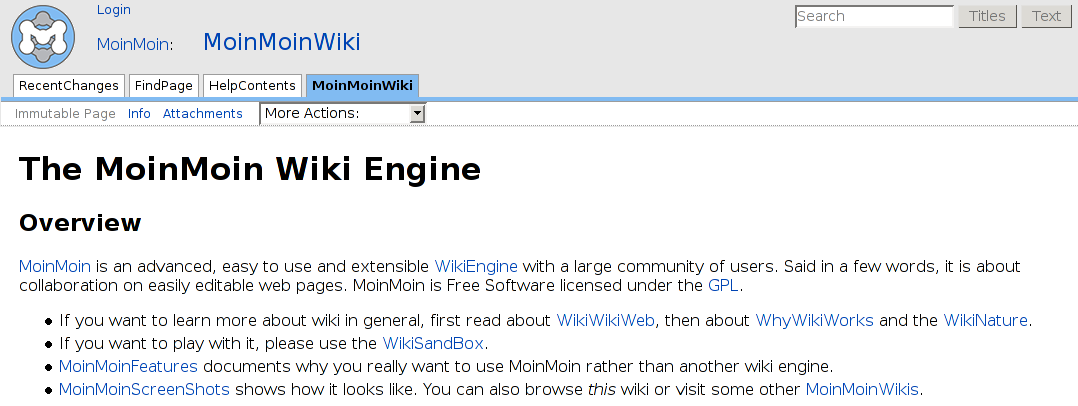
\includegraphics[height=4cm]{images/moinmoin.png}
\end{frame}

\begin{frame}[fragile]
\frametitle{NumPy + SciPy + Matplotlib = Pylab}
Ein Ersatz f"ur MatLab: Matritzenrechnung, numerische Funktionen, Plotten, ...

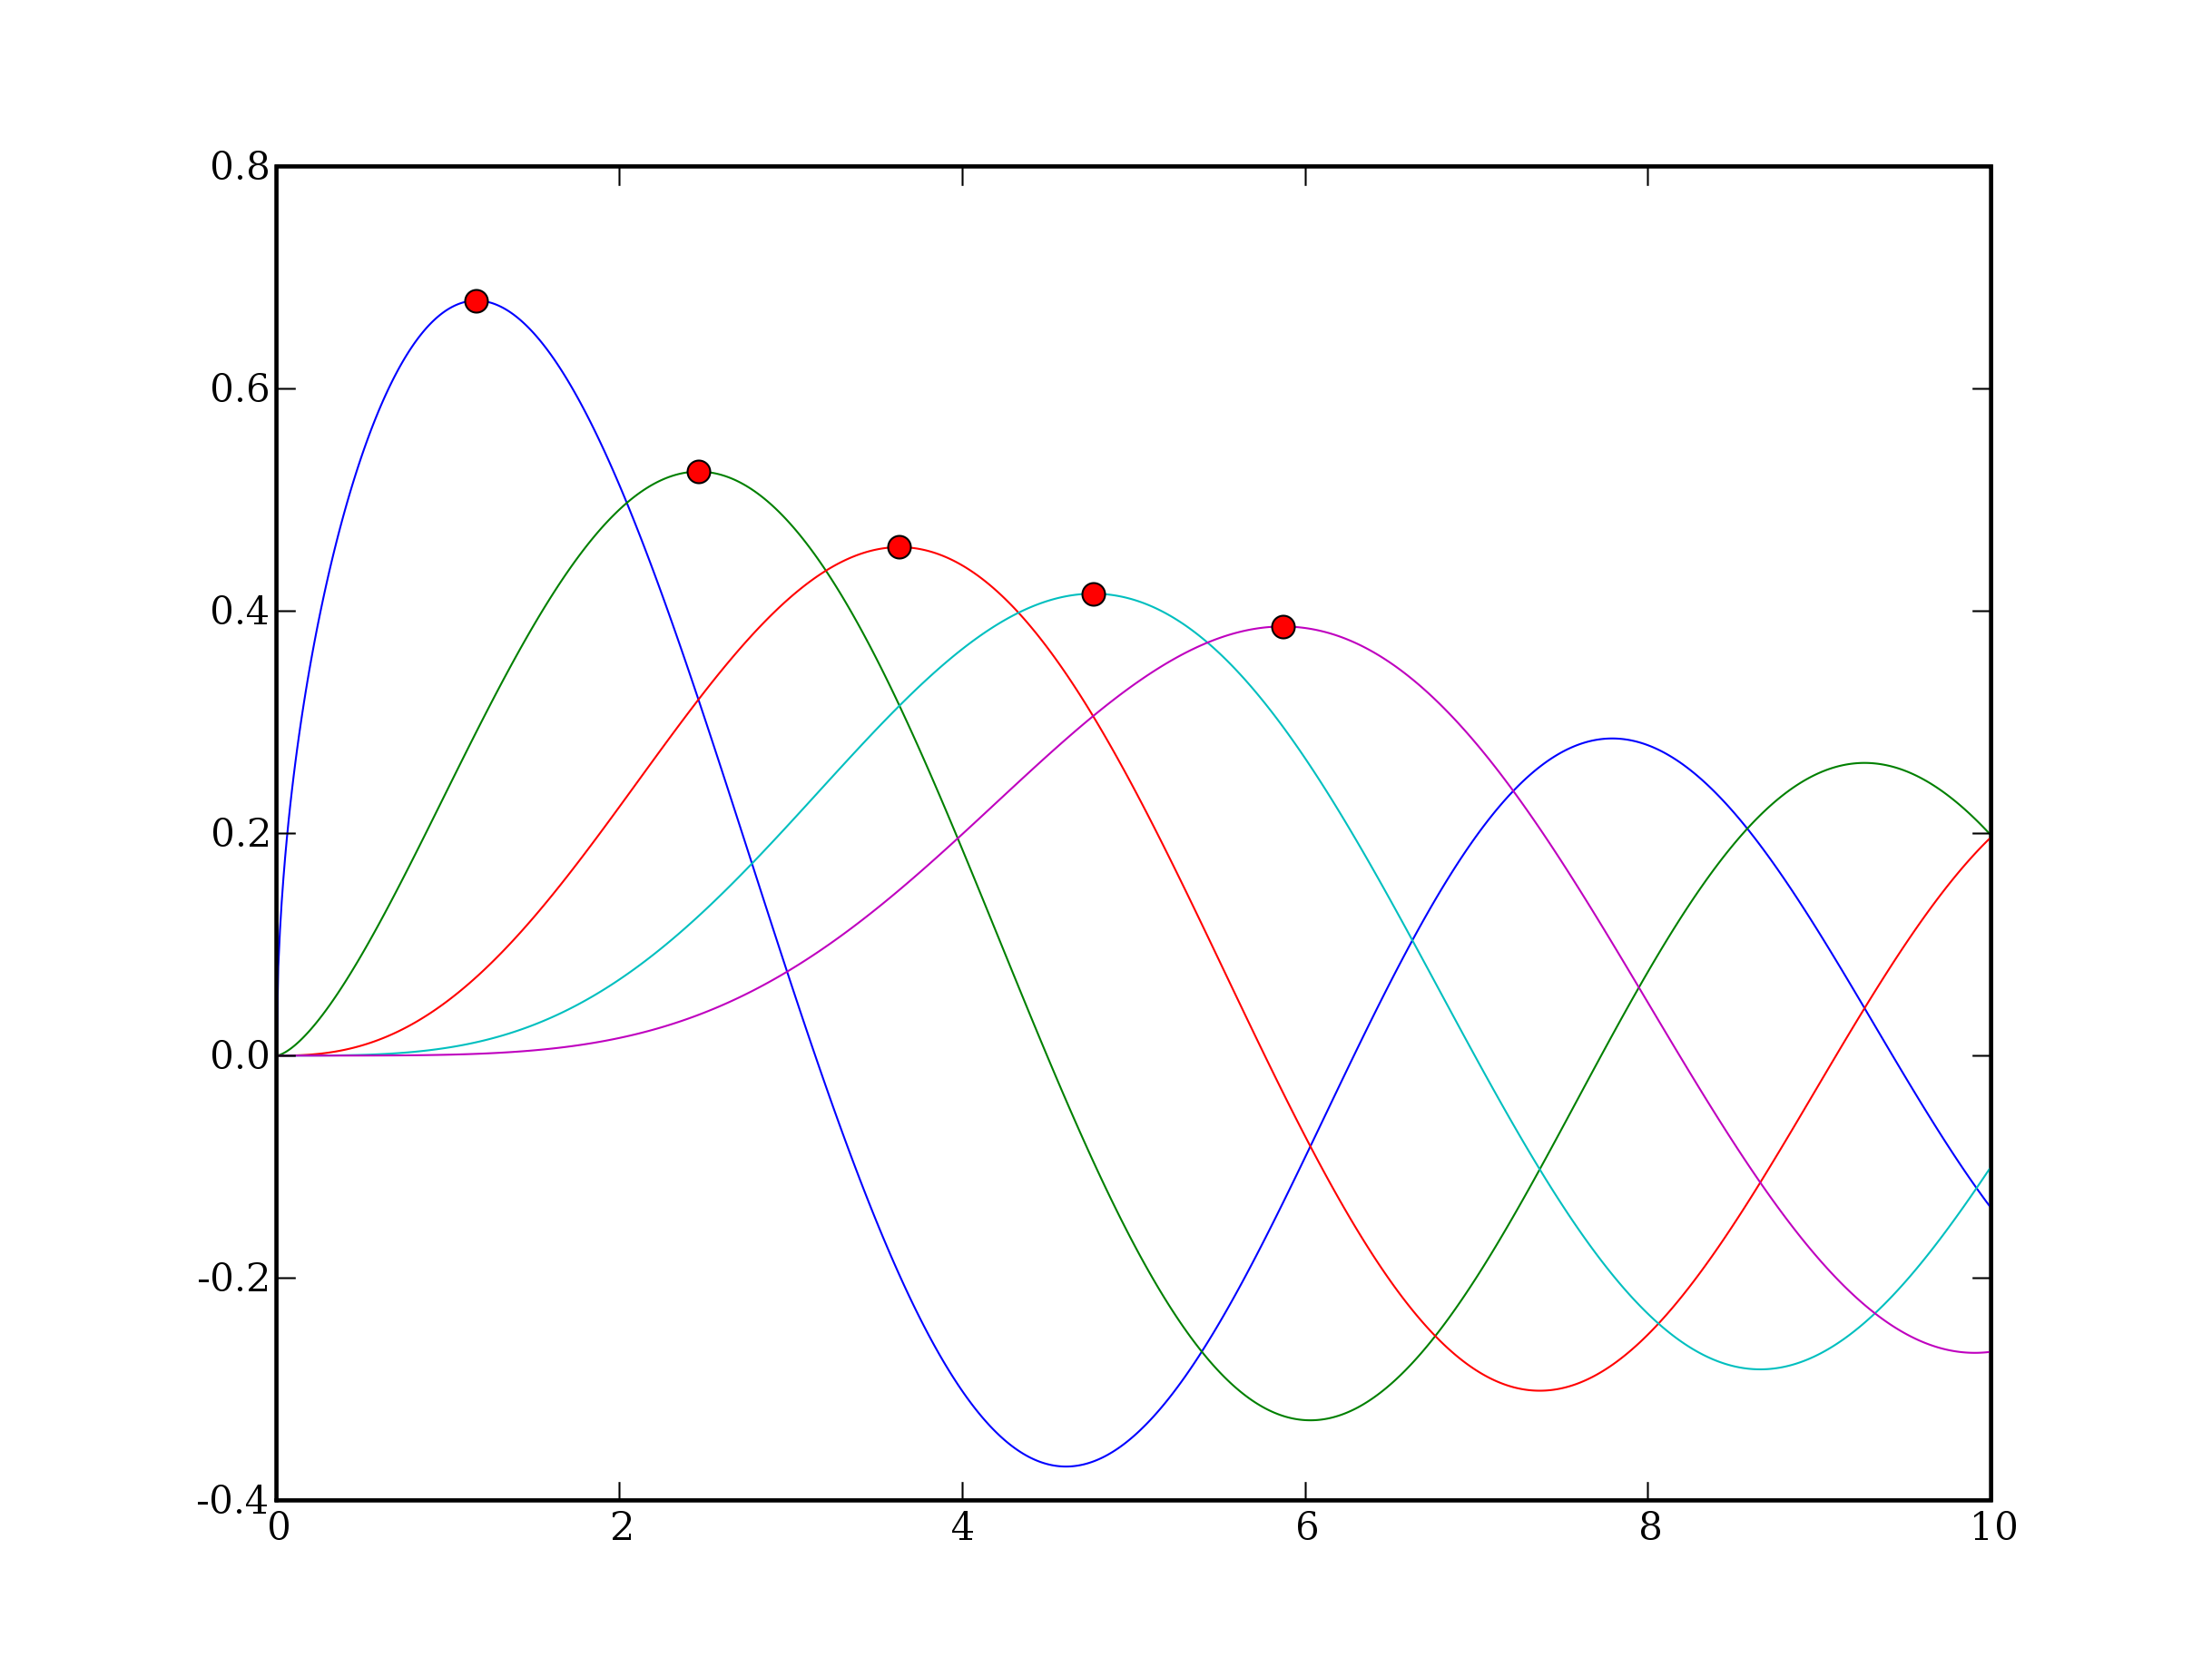
\includegraphics[height=4cm]{images/matplotlib.png}
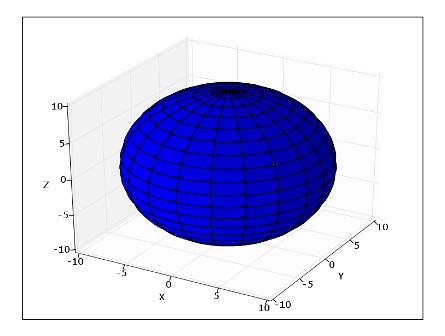
\includegraphics[height=4cm]{images/surface.jpg}

\begin{lstlisting}[style=Python, basicstyle=\small]
A = matrix([[1, 2], [2, 1]]); b = array([1, -1])
matshow(A)
(eigvals, eigvecs) = eig(A)
x = linalg.solve(A, b)
\end{lstlisting}
\end{frame}

%%% Local Variables: 
%%% mode: latex
%%% latex-run-command: pdflatex
%%% TeX-master: "vortrag"
%%% End: 
